We adapted algorithms in \cite{vamplew_potential-based_2021}, comparing the existing \tloA{} aggregation function with several new aggregation and scalarization functions. These were compared using the same environments and benchmarks as in \cite{vamplew_potential-based_2021}. Specifically, the environments were the UnbreakableBottles (UB) environment, the BreakableBottles (BB) environment, the Sokoban environment, and the Doors environment.
\subsection{Testing environment}

We used a modified version of the testing environment from \cite{vamplew_potential-based_2021}, obtained with permission from the authors. Learning proceeded for 5,000 episodes, and performance during learning (online performance) and after learning (offline performance) was measured. There were several key changes for our implementation. Changes affecting modeling results themselves are described below. Each experimental condition itself run for 100 trials in order to build up a probability distribution, making the comparison results generalisable to repeated runs of the task.



\subsubsection{Aggregation functions}



All of the multi-objective utility functions we compared use the following steps: 
\begin{enumerate}
    \item %When reinforcement occurs from the environment,
    A scaling factor $c_i$ is applied to each objective, specific to that reinforcement, by multiplying it with the value of reinforcement at each time point. This step has not been implemented in this paper but we emphasize its possible use in the future. \footnote{Clarify:  I think if the step is included here it needs to describe something we're actually doing in this experiment, or at least, we need to spell out that it's not actually used here--unless it is?}
    \item Transform the scaled output of  using a non-linear transform, as described below (Figure~\ref{fig:transform_functions} and Figure ~\ref{fig:seba_transform_functions_3d}). %For SFMLA, SFELLA, ELA, LELA, and SEBA, the transform is applied independently for each objective. % this is for ALL of the studied functions, right?
    
    \item Combine the transformed output using a simple average/sum as in Equation~\ref{eq:meu}.
\end{enumerate}

These steps describe a value function which can be applied either to the individual reinforcement delivered at each in response to an action, or to Q-values during action selection. In Experiment 1, we apply these steps to Q-values during action selection.

Each non-linear function is applied component-wise before aggregation occurs by averaging/summing of the transformed values

\begin{align}
\label{eq:meu}
U=\sum_{i}^n{f_i(c_i x_i)}
\end{align}

\noindent where ${f_i}$ describes a specific transform function for the $i$th objective, explained in more detail below. Note that here, $U$ describes our modeling of Q-values. The scaling factors $c_i$ can be treated as parameters of the model. They could be, for example, specified directly by the human, automatically determined in the future by the agent using a value learning method, or calculated by some other algorithm. 
For the purposes of this experiment, we left these at $c=1$ (instead, we directly modified $x$, the value returned by the environment), but emphasize that modifying these scale values could be useful in the future.


 New non-linear transforms compared are:

\begin{itemize}
    %\item Split-function multiplicative loss aversion (SFMLA)
    \item Split-function exp-log loss aversion (SFELLA)
    \item Exponential loss aversion (ELA)
    \item Linear-exponential loss aversion (LELA)
    \item Squared error based alignment (SEBA)
\end{itemize}

\noindent The SEBA transform function envisages differing functions for `primary' and `alignment' categories of objectives. All other transform functions do not distinguish categories of objectives, and apply the same function over all objectives.

Each non-linear transform is a transform of the value obtained along a specific objective %$O$
at a specific state %$s$ 
with a specific action %$a$\footnote{need to decide how much of this notation we include. If we include it, need to rewrite formulae to reflect it. Might take some inspiration from Vamplew's earlier papers. Should almost certainly be giving a formula for $TLO^A$}. 
The SFELLA, ELA, and LELA functions are illustrated in Figure~\ref{fig:transform_functions}. The SEBA aggregation is illustrated on Figure ~\ref{fig:seba_transform_functions_3d}.

For each transform, where $x=0$, $f(x)=0$. This is a minor modification from the non-linear transform previously proposed in \cite{rolf_need_2020}, typically achieved by adding 1 to the outcome value.

Each function also provides that $\frac{\mathrm{d} f(x) }{\mathrm{d} x}$ declines as $x$ gets larger. This lowers inequality between outcomes as measured in different objectives, objectives where values are strongly negative get disproportionately higher priority. Where different objectives were operationalizing, for instance, priorities among different interested parties, this might be particularly useful in reducing inequality between outcomes.



\begin{figure*}[h]
 
  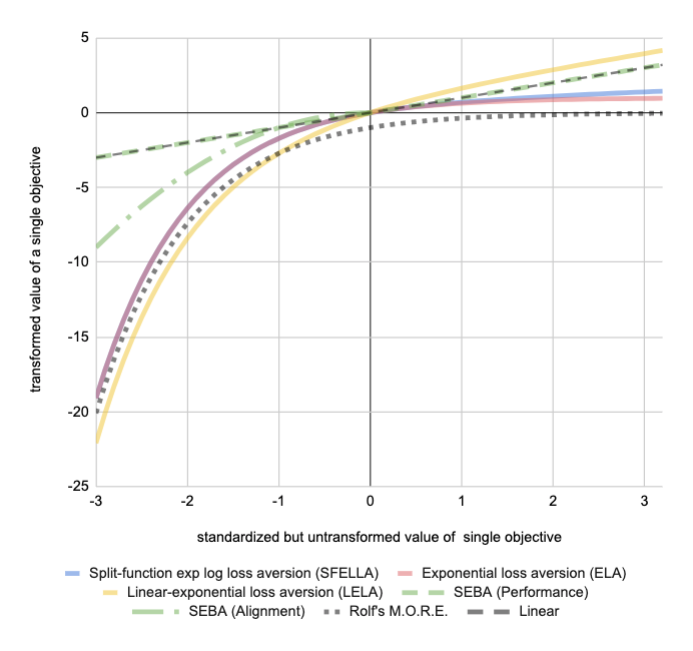
\includegraphics[width=\columnwidth]{output/transform_graph-2d_with_rolf2.png}%\footnote{Roland: Can you please add the -x*x from SEBA to the left part of the plots too? Maybe using some short-dashed line for example. It would illustrate that the square function is less steep than the exponential functions, thus being in between linear and exponential}
  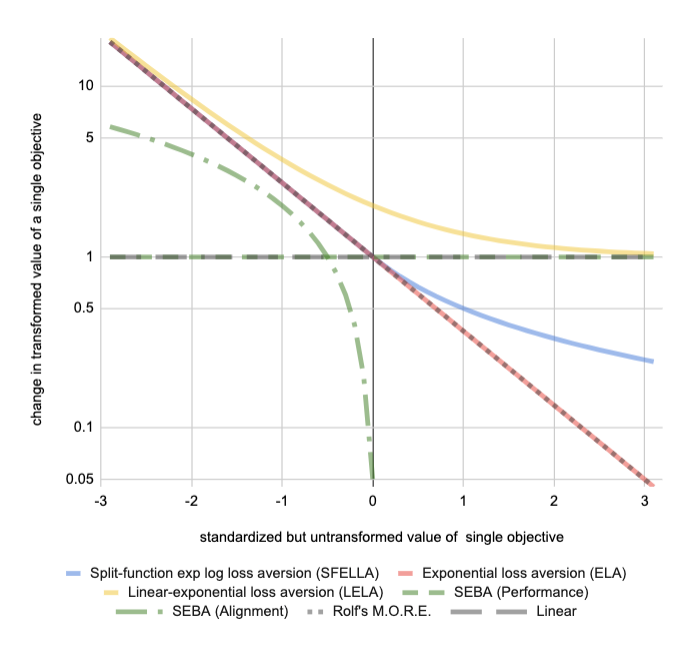
\includegraphics[width=\columnwidth]{output/transform_graph_2d_integral_with_rolf2.png}%\footnote{Roland: I would add comment that the the y scale is log scale, otherwise this plot is confusing, until one looks at the numbers at the left side}
  \caption{Transform functions. Left: Each transform function is applied to the utility received from the environment for each objective, or to the Q value of the RL agent for each objective. In our current setup it is applied to the Q values of the RL agent.
  %\footnote{why repeat the same thing when you can leave out the other option?}. 
  The output of each of these transform functions are averaged together % in a Maximize Expected Utility Model \footnote{if anything this should be called MOMEU, right?}
  (Equation~\ref{eq:meu}). %\rk{Should we include a min function here, to show the soft minimax characteristic?} 
  Right: Change in $f(x)$ per unit $x$, with $y$ axis plotted on a log scale%\footnote{could be omitted}
  . Note that ELA and SFELLA produce greater-than-linear change in $f(x)$ when $x<0$ and less-than-linear change when $x>0$. In contrast, LELA's change never falls below 1.}
  \label{fig:transform_functions}
  \Description{Transform functions.}
\end{figure*}

\begin{figure*}[h]
 
  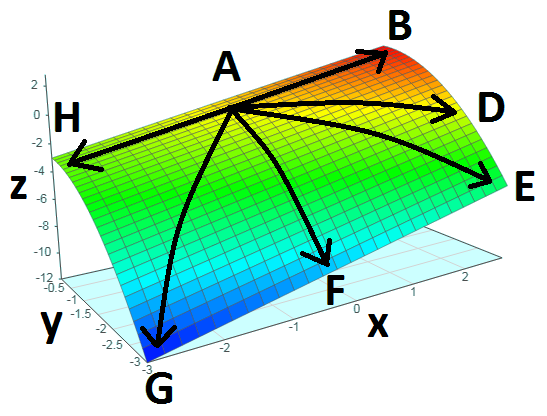
\includegraphics[width=\columnwidth]{output/seba1b.png}
  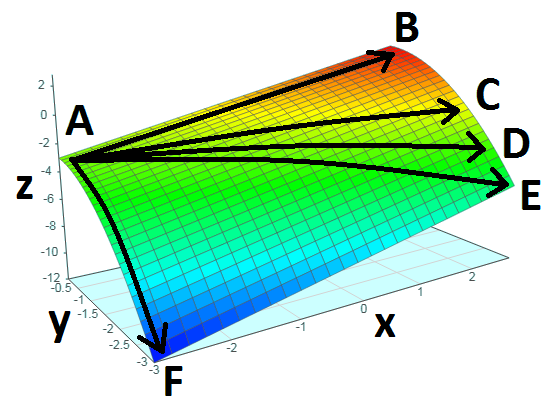
\includegraphics[width=\columnwidth]{output/seba2b.png}
  \caption{Transform for the SEBA aggregation. One of the objectives is the alignment objective (the y-axis), and the other objective is the performance objective (the x-axis). The z-axis represents the aggregated utility. The two types of objectives are treated differently. The performance objective has always linear treatment regardless of the current sign of its input measure, while the alignment measure is upper-bounded at zero and has exponential treatment (in case of SEBA it is a negated squared error). These plots illustrate two things. 1. The performance objective (the x-axis) is linear regardless of the sign of the value of the input measure. 2. The alignment related measure (the y-axis) may be sacrificed, but only up to a degree. Once alignment would be sacrificed too much, the evaluation of the aggregated utility quickly becomes strongly negative, since the alignment measure is treated exponentially. So this provides the loss aversion aspect.}
  \label{fig:seba_transform_functions_3d}
  \Description{Transform for the SEBA aggregation.}
\end{figure*}

%SFMLA might be the function that most intuitively expresses loss aversion, the idea that losses loom larger than gains:

%\begin{align}
%U^P(s, a)'= & cU^P(s, a) & \mathrm{ where \: U^P(s, a)>0} \\ \nonumber
%  &  2c U^P(s, a) &  \mathrm{otherwise} \\ \nonumber
%\end{align}

%(or we can write the following; which is better?)

%\begin{align}
%f(x)= & cx & \mathrm{ where \: x>0} \\ \nonumber
%  & 2c x &  \mathrm{otherwise} \\ \nonumber
%\end{align}

In SFELLA, there is a split in the function at $x=0$. It expresses a loss-averse function where losses will be amplified more than gains:

\begin{align}
f(x)= & \ln(cx+1) & \mathrm{ where \: x>0} \\ \nonumber
  &  -\exp(-cx)+1 &  \mathrm{otherwise} \\ \nonumber
\end{align}

Additionally, by implementing a log rather than a negative exponential in the positive domain, the function retains relatively more weight on positive objectives, i.e. is not bounded.

The ELA is a simplification of this without a case distinction at the cost of giving very little weight to any increase in values over 1:

\begin{align}
f(x)= &  -\exp(-cx)+1 \\ \nonumber
\end{align}

With LELA we add a $x$ term so that value continues to increase at least linearly for large inputs:

\begin{align}
f(x)= &  -\exp(-cx)+cx+1 \\ \nonumber
\end{align}

This still yields loss aversion at points less than zero but always provides that an increase in $x$ increases at least linearly in $f(x)$%\footnote{sound repetitive}.


Finally, SEBA takes a different approach in that rather than treating each objective identically, transformations are applied differently to performance and alignment objectives.%\footnote{earlier this was called a safety objective}.

For performance objectives the SEBA formula is linear:
\begin{align}
f(x)= &  cx \\ \nonumber
\end{align}
There is no differentiation between negative and positive areas of the measures of the performance objectives. This avoids the need for establishing a zero-point. Proper scaling is still needed.

SEBA expresses loss aversion for alignment objectives using a negated square power function, and assumes that alignment objectives are non-positive:
\begin{align}
\label{eq:seba}
f(x)= &  -(cx)^2 \\ \nonumber
  &  \mathrm{ where \: x \leq 0}
\end{align}

The alignment related measures still have a “natural” zero-point, since they by definition are bounded at zero where no (soft) constraint violations are occurring. %Therefore in case of safety related features it is not so difficult to establish where the zero-point is located at. 
Such measures would usually measure the deviation of something from a desired target value. Such measures have two main types:
\begin{itemize}
    \item The desired target value is zero (for example, zero harm, etc).
    \item Alternatively it might be a homeostatic set-point (for example, optimal temperature, etc), so the measure is representing the negated absolute value of the deviation regardless of the direction of the deviation.
\end{itemize}
The SEBA aggregation is illustrated on Figure ~\ref{fig:seba_transform_functions_3d}. A number of specific situations are illustrated in the graph using upper-case letter points, and it is helpful to consider their interpretation:
  \begin{itemize}
      \item A - The initial state. The alignment objective / soft constraint is met and the performance objective is either at zero (left side plot) or at negative value (right side plot).
      \item B - The performance objective is improved, the alignment constraint is preserved. Moving in this direction changes the aggregated score linearly thus enabling independence from the zero-point.
      \item C - Shown only on the right side plot. Performance objective is improved significantly, while alignment constraint is sacrificed just so slightly that the aggregated utility is still improved.
      \item D - Performance objective is improved significantly, but the alignment constraint is sacrificed so much that the aggregated utility does not change as compared to the initial state. The agent is neutral to this state change and is not driven towards this state nor avoiding it.
      \item E - Performance objective is improved significantly, while the alignment constraint is violated significantly. Therefore the aggregated utility becomes worse than the initial state. The agent avoids this state.
      \item F - The measure for the performance objective does not change, but the alignment constraint gets violated.
      \item G - Shown only on the left side plot. Both the performance objective and the alignment objective / constraint get worse.
      \item H - Shown only on the left side plot. The performance objective gets much worse but the alignment constraint is still satisfied. It is also noteworthy that this state is evaluated to be about as good as the alternative state somewhere between D and E where the alignment constraint is getting notably violated but the performance objective is improved much.
  \end{itemize}

\subsubsection{Environment}

In every environment, agents have two objectives: a `performance' objective (denoted \RP{}) and an `alignment' objective (denoted \RA{}). %\footnote{need to standarize terms. are we using primary or performance or reward; impact or alignment or penalty; etc - Roland: I vote for performance objective and alignment objective. These terms are in use also in Vamplew's code. It seems to be also important to avoid using the phrase "primary" objective as it is quite misleading in our context, since in practice the alignment objective is stronger and therefore sort of more primary. The word "reward" can remain where it is appropriate, since it is a measure, a proxy for the objective.} 
Four gridworld environments reported in \cite{vamplew_potential-based_2021} were examined.
They are shown in \ref{fig:envs} and we call them the 'Breakable and Unbreakable Bottles' (BB and UB), 'Sokoban' and 'Doors'.

The Bottles environments share the same 1D grid layout where one end is the destination 'D' where the agent has to deliver bottles and the other end is the source 'S' where bottles are provided.
Initially, the agent does not carry a bottle and it can hold up to two bottles and an episode ends when two bottles have been delivered.
While in between source and destination an agent holding two bottles can drop a bottle on a tile with a probability of 10\%.
Leaving a bottle on the way yields a penalty of -50 in R$^*$.
While in UnbreakableBottles the bottles can be picked up again where they were left, in BreakableBottles they break upon dropping hence irreversibly changing the environment and receiving the penalty.

In the Sokoban environment the agent starts on tile 'S' and is tasked with pushing away the box 'B' in order to reach the goal tile 'G'.
There are two ways of pushing: downwards into a corner (irreversible) and to the left (reversible, but involving more steps).
A penalty of -25 is evoked for each wall touching the box in the final position.

In the Doors environment the agent must simply travel from the start 'S' to the goal 'G'.
It can choose to open or close the doors (grey) which takes each one action. 
There are two possible paths: either the agent can move around the right corridor taking 10 moves to reach 'G' or the agent can move straight down by opening the doors (6 moves if the doors stay open).
However, there is a penalty of -10 associated with leaving a door open.
Therefore the desired solution is moving down while closing the doors behind the agent taking 8 moves.

We wanted to understand how different aggregation functions could respond to re-scaling of primary or alignment rewards. To do this, we repeated each experiment 9 times. The first time was with the original settings as in \cite{vamplew_potential-based_2021}. Then, we repeated this with each environment's primary objective feedback scaled by $10^{-2}$, $10^{-1}$, $10^1$, and $10^2$. The same range of scaling was then applied to the alignment objective feedback. This scaling could in some scenarios potentially be distinguished from $c$ in Equations~\ref{eq:meu}-\ref{eq:seba}. Even though it is mathematically equivalent in our implementation, it could represent changes to the environment rather than changes in agent evaluation.


\begin{figure}
    \centering
    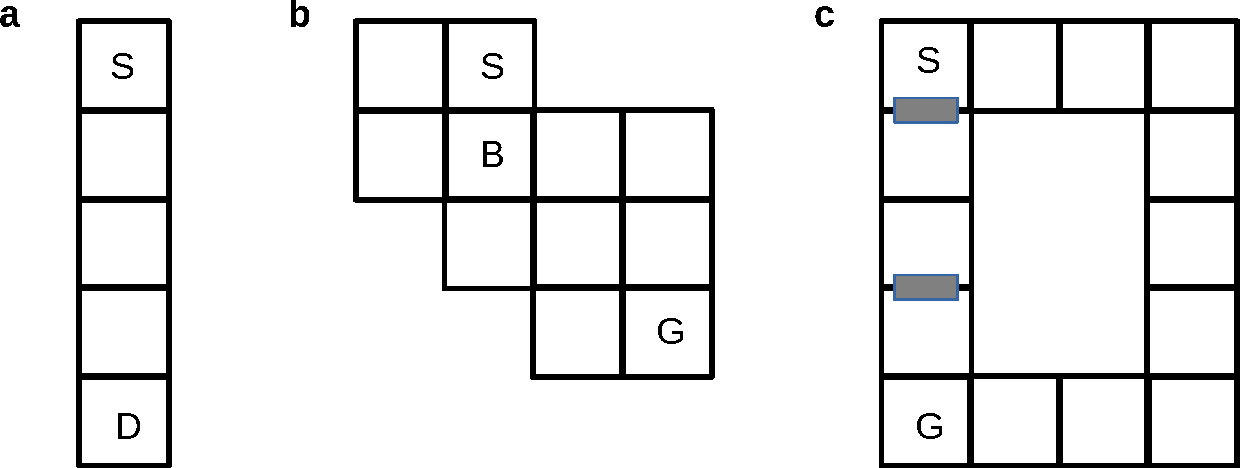
\includegraphics[width=1\columnwidth]{output/env_figure.pdf}
    \caption{Maps of physical environments in (a) (Un)Breakable Bottles, (b) Sokoban, (c) Doors. Based on Figure in \cite{vamplew_potential-based_2021}.}
    \label{fig:envs}
\end{figure}

\subsubsection{Measurement}

Each of the proposed functions was compared against the best performing function in \cite{vamplew_potential-based_2021}, the \tloA{} function, on the `R$^*$' metric from the same paper. The `R$^*$' arbitrarily scores a weighted combination of Performance and alignment objectives where one unit of alignment objective (always on a negative scale) is worth 10-50 units of the Performance objective, depending on the environment.%\footnote{Roland: The ratio of units is somewhat different across environments. It is not always 50 units. Vamplew paper describes the details. I think the range was about 10 to 50.}

Learning was switched off after 5000 episodes. Following that time, offline performance was observed as the average across offline performance in all 100 runs.

